% (find-LATEX "2021-1-C3-MT2.tex")
% (defun c () (interactive) (find-LATEXsh "lualatex -record 2021-1-C3-MT2.tex" :end))
% (defun C () (interactive) (find-LATEXsh "lualatex 2021-1-C3-MT2.tex" "Success!!!"))
% (defun D () (interactive) (find-pdf-page      "~/LATEX/2021-1-C3-MT2.pdf"))
% (defun d () (interactive) (find-pdftools-page "~/LATEX/2021-1-C3-MT2.pdf"))
% (defun e () (interactive) (find-LATEX "2021-1-C3-MT2.tex"))
% (defun o () (interactive) (find-LATEX "2021-1-C3-MT1.tex"))
% (defun u () (interactive) (find-latex-upload-links "2021-1-C3-MT2"))
% (defun v () (interactive) (find-2a '(e) '(d)))
% (defun d0 () (interactive) (find-ebuffer "2021-1-C3-MT2.pdf"))
% (defun cv () (interactive) (C) (ee-kill-this-buffer) (v) (g))
%          (code-eec-LATEX "2021-1-C3-MT2")
% (find-pdf-page   "~/LATEX/2021-1-C3-MT2.pdf")
% (find-sh0 "cp -v  ~/LATEX/2021-1-C3-MT2.pdf /tmp/")
% (find-sh0 "cp -v  ~/LATEX/2021-1-C3-MT2.pdf /tmp/pen/")
%     (find-xournalpp "/tmp/2021-1-C3-MT2.pdf")
%   file:///home/edrx/LATEX/2021-1-C3-MT2.pdf
%               file:///tmp/2021-1-C3-MT2.pdf
%           file:///tmp/pen/2021-1-C3-MT2.pdf
% http://angg.twu.net/LATEX/2021-1-C3-MT2.pdf
% (find-LATEX "2019.mk")
% (find-CN-aula-links "2021-1-C3-MT2" "3" "c3m211mt2" "c3mt2")
%
% Video (not yet):
% (find-ssr-links "c3m211mt2" "2021-1-C3-MT2")
% (code-video     "c3m211mt2video" "$S/http/angg.twu.net/eev-videos/2021-1-C3-MT2.mp4")
% (find-c3m211mt2video "0:00")

% «.defs»	(to "defs")
% «.title»	(to "title")
% «.gabarito»	(to "gabarito")
%
% «.djvuize»	(to "djvuize")

\documentclass[oneside,12pt]{article}
\usepackage[colorlinks,citecolor=DarkRed,urlcolor=DarkRed]{hyperref} % (find-es "tex" "hyperref")
\usepackage{amsmath}
\usepackage{amsfonts}
\usepackage{amssymb}
\usepackage{pict2e}
\usepackage[x11names,svgnames]{xcolor} % (find-es "tex" "xcolor")
\usepackage{colorweb}                  % (find-es "tex" "colorweb")
%\usepackage{tikz}
%
% (find-dn6 "preamble6.lua" "preamble0")
%\usepackage{proof}   % For derivation trees ("%:" lines)
%\input diagxy        % For 2D diagrams ("%D" lines)
%\xyoption{curve}     % For the ".curve=" feature in 2D diagrams
%
\usepackage{edrx21}               % (find-LATEX "edrx21.sty")
\input edrxaccents.tex            % (find-LATEX "edrxaccents.tex")
\input edrx21chars.tex            % (find-LATEX "edrx21chars.tex")
\input edrxheadfoot.tex           % (find-LATEX "edrxheadfoot.tex")
\input edrxgac2.tex               % (find-LATEX "edrxgac2.tex")
%
%\usepackage[backend=biber,
%   style=alphabetic]{biblatex}            % (find-es "tex" "biber")
%\addbibresource{catsem-slides.bib}        % (find-LATEX "catsem-slides.bib")
%
% (find-es "tex" "geometry")
\usepackage[a6paper, landscape,
            top=1.5cm, bottom=.25cm, left=1cm, right=1cm, includefoot
           ]{geometry}
%
\begin{document}

\catcode`\^^J=10
\directlua{dofile "dednat6load.lua"}  % (find-LATEX "dednat6load.lua")

%L dofile "edrxtikz.lua"     -- (find-LATEX "edrxtikz.lua")
%L dofile "edrxpict.lua"     -- (find-LATEX "edrxpict.lua")
%L -- dofile "2021-1-C3-3D.lua" -- (find-LATEX "2021-1-C3-3D.lua")
%L -- V3.__index.tostring = function (v) return v:v2string() end
\pu

% «defs»  (to ".defs")
% (find-LATEX "edrx15.sty" "colors-2019")
%\long\def\ColorRed   #1{{\color{Red1}#1}}
%\long\def\ColorViolet#1{{\color{MagentaVioletLight}#1}}
%\long\def\ColorViolet#1{{\color{Violet!50!black}#1}}
%\long\def\ColorGreen #1{{\color{SpringDarkHard}#1}}
%\long\def\ColorGreen #1{{\color{SpringGreenDark}#1}}
%\long\def\ColorGreen #1{{\color{SpringGreen4}#1}}
%\long\def\ColorGray  #1{{\color{GrayLight}#1}}
%\long\def\ColorGray  #1{{\color{black!30!white}#1}}
%\long\def\ColorBrown #1{{\color{Brown}#1}}
%\long\def\ColorBrown #1{{\color{brown}#1}}
%\long\def\ColorOrange#1{{\color{orange}#1}}
%
%\long\def\ColorShort #1{{\color{SpringGreen4}#1}}
%\long\def\ColorLong  #1{{\color{Red1}#1}}
%
%\def\frown{\ensuremath{{=}{(}}}
%\def\True {\mathbf{V}}
%\def\False{\mathbf{F}}
%\def\D    {\displaystyle}

\def\drafturl{http://angg.twu.net/LATEX/2021-1-C3.pdf}
\def\drafturl{http://angg.twu.net/2021.1-C3.html}
\def\draftfooter{\tiny \href{\drafturl}{\jobname{}} \ColorBrown{\shorttoday{} \hours}}



%  _____ _ _   _                               
% |_   _(_) |_| | ___   _ __   __ _  __ _  ___ 
%   | | | | __| |/ _ \ | '_ \ / _` |/ _` |/ _ \
%   | | | | |_| |  __/ | |_) | (_| | (_| |  __/
%   |_| |_|\__|_|\___| | .__/ \__,_|\__, |\___|
%                      |_|          |___/      
%
% «title»  (to ".title")
% (c3m211mt2p 1 "title")
% (c3m211mt2a   "title")

\thispagestyle{empty}

\begin{center}

\vspace*{1.2cm}

{\bf \Large Cálculo 3 - 2021.1}

\bsk

Mini-teste 2

\bsk

Eduardo Ochs - RCN/PURO/UFF

\url{http://angg.twu.net/2021.1-C3.html}

\end{center}

\newpage

{\bf Regras}

As regras vão ser as mesmas dos

mini-testes do semestre passado:

\ssk

{\footnotesize

\url{http://angg.twu.net/LATEX/2020-2-C2-MT1.pdf#page=2}

}

\bsk

\ColorRed{Leia com muita atenção!!!!!!!!!!!}


\bsk
\bsk

As questões vão ser disponibilizadas às 20:00 da sexta

27/agosto/2021 e vocês vão ter até as 20:00 do sábado

28/agosto/2021 pra entregar as respostas.

\msk

Este mini-teste vale 0.5 pontos a mais na P1.


\newpage

{\bf Questão 1 (e única).}

Esta questão é exatamente equal à que começamos

a fazer na aula antes do mini-teste...

\ssk

% (c3m211jp 7 "preparacao-mini-teste")
% (c3m211ja   "preparacao-mini-teste")

{\footnotesize

% (c3m211jp 7)
%    http://angg.twu.net/LATEX/2021-1-C3-matriz-jacobiana.pdf#page=7
\url{http://angg.twu.net/LATEX/2021-1-C3-matriz-jacobiana.pdf#page=7}

}

...mas com um desenho um pouquinho mais complicado.

\ssk

Descubra qual a imagem da figura abaixo pela função

$z \mapsto z^2$ e faça um desenho razoavelmente preciso dela.
%
% (find-latexscan-links "C3" "20210827_9+4_quadrados")
% (find-xpdf-page "~/LATEX/2021-1-C3/20210827_9+4_quadrados.pdf")
$$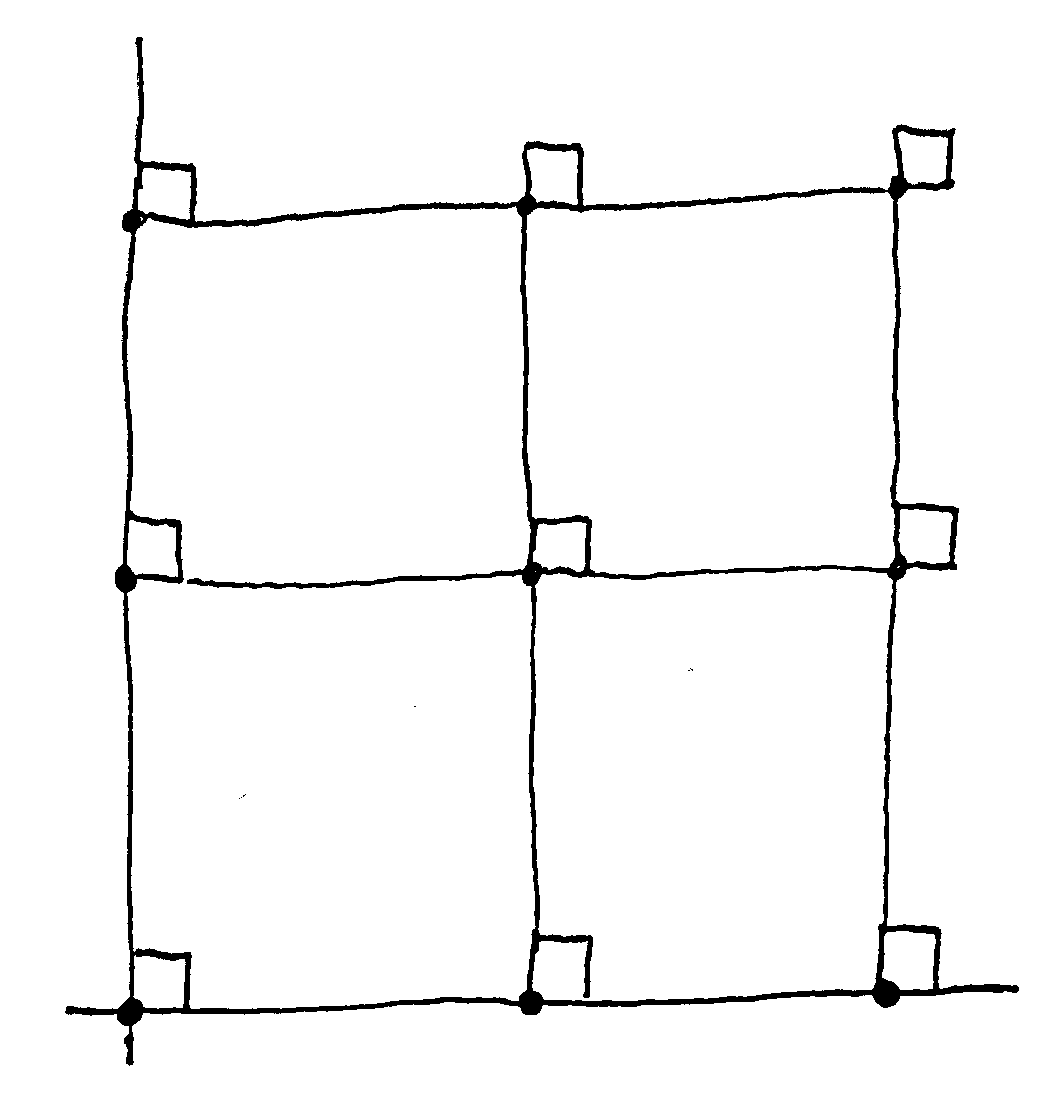
\includegraphics[height=3.5cm]{2021-1-C3/20210827_9+4_quadrados.pdf}$$


\newpage

% «gabarito»  (to ".gabarito")
% (c3m211mt2p 4 "gabarito")
% (c3m211mt2a    "gabarito")

{\bf Gabarito}

(Usei $a=b=0.2$)
%
\unitlength=15pt
%
%L complexsquare = function (a, b)
%L     return a*a - b*b, 2*a*b
%L   end
%L csq = function (vv)
%L     return v(complexsquare(vv[1], vv[2]))
%L   end
%L drawsquare = function (vv, f, e)
%L     return pformat("\\polygon%s%s%s%s",
%L                    f(vv), f(vv+v(e,0)), f(vv+v(e,e)), f(vv+v(0,e)))
%L   end
%L drawline = function (vv, ww, f, n)
%L     local g = function (k) return tostring(f(tow(vv, ww, k/n))) end
%L     return "\\Line"..mapconcat(g, seq(0, n), "")
%L   end
%L drawall = function (f, eps, n)
%L     return table.concat({
%L       drawsquare(v(0, 0), f, eps),
%L       drawsquare(v(0, 1), f, eps),
%L       drawsquare(v(0, 2), f, eps),
%L       drawsquare(v(1, 0), f, eps),
%L       drawsquare(v(1, 1), f, eps),
%L       drawsquare(v(1, 2), f, eps),
%L       drawsquare(v(2, 0), f, eps),
%L       drawsquare(v(2, 1), f, eps),
%L       drawsquare(v(2, 2), f, eps),
%L       drawline(v(0, 0), v(0, 2), f, n),
%L       drawline(v(1, 0), v(1, 2), f, n),
%L       drawline(v(2, 0), v(2, 2), f, n),
%L       drawline(v(0, 0), v(2, 0), f, n),
%L       drawline(v(0, 1), v(2, 1), f, n),
%L       drawline(v(0, 2), v(2, 2), f, n),
%L       }, "\n")
%L   end
\pu
%
$$\vcenter{\hbox{%
    \beginpicture(-1,-1)(3,3)
    \pictgrid%
    {\linethickness{1.251pt}%
     \expr{drawall(id, 0.2, 1)}%
    }
    \pictaxes%
    \end{picture}%
  }}
  \quad
  \mapsto
  \quad
  \vcenter{\hbox{%
    \beginpicture(-6,-1)(6,10)
    \pictgrid%
    {\linethickness{1.25pt}%
     \expr{drawall(csq, 0.2, 10)}%
    }
    \pictaxes%
    \end{picture}%
  }}
$$

\newpage

{\bf Um jeito de fazer as contas}
%
\def\Lxx#1{\lim_{Δx→0} \frac{#1}{Δx}}
\def\Lyy#1{\lim_{Δy→0} \frac{#1}{Δy}}
%
$$\scalebox{0.9}{$
  \begin{array}{rcl}
  w_x &=& \D \Lxx {w(x_0+Δx,y_0) - w}                      \\[7pt]
      &=& \D \Lxx {(a(x_0+Δx,y_0), b(x_0+Δx,y_0)) - (a,b)} \\[7pt]
      &=& \D \Lxx {(a + a_x Δx, b + b_x Δx) - (a,b)}       \\[7pt]
      &=& \D \Lxx {(a_x Δx, b_x Δx)}                       \\[7pt]
      &=& \D \Lxx {(a_x, b_x) Δx}                          \\[7pt]
      &=& \VEC{a_x, b_x}                                   \\[7pt]
  w_y &=& \D \Lyy {w(x_0,y_0+Δy) - w}                      \\[7pt]
      &=& \VEC{a_y, b_y}                                   \\[7pt]
  \end{array}
  $}
$$

\newpage

\vspace*{-0.5cm}

$$w = (a,b) = (x^2 - y^2, 2xy)$$
$$w_z = \frac{d\psm{a\\b}}{d\psm{x\\y}}
      = \pmat{a_x & a_y \\ b_x & b_y}
      = \pmat{2x & -2y \\ 2y & 2x}
$$
$$w_x = \VEC{a_x, b_x} = \VEC{2x, 2y}$$
$$w_y = \VEC{a_y, b_y} = \VEC{-2y, 2x}$$

Em $(x,y) = (2,0)$ temos $w=(4,0)$, $w_x=\VEC{4,0}$, $w_y=\VEC{0,4}$

Em $(x,y) = (2,1)$ temos $w=(3,4)$, $w_x=\VEC{4,2}$, $w_y=\VEC{-2,4}$

Em $(x,y) = (2,2)$ temos $w=(0,8)$, $w_x=\VEC{4,4}$, $w_y=\VEC{-4,4}$

Em $(x,y) = (1,2)$ temos $w=(-3,4)$, $w_x=\VEC{2,4}$, $w_y=\VEC{-4,2}$

\msk

$w(1.2, 2) ≈ w(1,2) + w_x(1,2)·0.2 = (-3,4) + 0.2·\VEC{2,4}$

$w(1, 2.2) ≈ w(1,2) + w_y(1,2)·0.2 = (-3,4) + 0.2·\VEC{-4,2}$

\GenericWarning{Success:}{Success!!!}  % Used by `M-x cv'

\end{document}

%  ____  _             _         
% |  _ \(_)_   ___   _(_)_______ 
% | | | | \ \ / / | | | |_  / _ \
% | |_| | |\ V /| |_| | |/ /  __/
% |____// | \_/  \__,_|_/___\___|
%     |__/                       
%
% «djvuize»  (to ".djvuize")
% (find-LATEXgrep "grep --color -nH --null -e djvuize 2020-1*.tex")

 (eepitch-shell)
 (eepitch-kill)
 (eepitch-shell)
# (find-fline "~/2021.1-C3/")
# (find-fline "~/LATEX/2021-1-C3/")
# (find-fline "~/bin/djvuize")

cd /tmp/
for i in *.jpg; do echo f $(basename $i .jpg); done

f () { rm -v $1.pdf;  textcleaner -f 50 -o  5 $1.jpg $1.png; djvuize $1.pdf; xpdf $1.pdf }
f () { rm -v $1.pdf;  textcleaner -f 50 -o 10 $1.jpg $1.png; djvuize $1.pdf; xpdf $1.pdf }
f () { rm -v $1.pdf;  textcleaner -f 50 -o 20 $1.jpg $1.png; djvuize $1.pdf; xpdf $1.pdf }

f () { rm -fv $1.png $1.pdf; djvuize $1.pdf }
f () { rm -fv $1.png $1.pdf; djvuize WHITEBOARDOPTS="-m 1.0 -f 15" $1.pdf; xpdf $1.pdf }
f () { rm -fv $1.png $1.pdf; djvuize WHITEBOARDOPTS="-m 1.0 -f 30" $1.pdf; xpdf $1.pdf }
f () { rm -fv $1.png $1.pdf; djvuize WHITEBOARDOPTS="-m 1.0 -f 45" $1.pdf; xpdf $1.pdf }
f () { rm -fv $1.png $1.pdf; djvuize WHITEBOARDOPTS="-m 0.5" $1.pdf; xpdf $1.pdf }
f () { rm -fv $1.png $1.pdf; djvuize WHITEBOARDOPTS="-m 0.25" $1.pdf; xpdf $1.pdf }
f () { cp -fv $1.png $1.pdf       ~/2021.1-C3/
       cp -fv        $1.pdf ~/LATEX/2021-1-C3/
       cat <<%%%
% (find-latexscan-links "C3" "$1")
%%%
}

f 20210827_9+4_quadrados

f 20201213_area_em_funcao_de_theta
f 20201213_area_em_funcao_de_x
f 20201213_area_fatias_pizza



%  __  __       _        
% |  \/  | __ _| | _____ 
% | |\/| |/ _` | |/ / _ \
% | |  | | (_| |   <  __/
% |_|  |_|\__,_|_|\_\___|
%                        
% <make>

 (eepitch-shell)
 (eepitch-kill)
 (eepitch-shell)
# (find-LATEXfile "2019planar-has-1.mk")
make -f 2019.mk STEM=2021-1-C3-MT2 veryclean
make -f 2019.mk STEM=2021-1-C3-MT2 pdf

% Local Variables:
% coding: utf-8-unix
% ee-tla: "c3mt2"
% ee-tla: "c3m211mt2"
% End:

